\documentclass[border=0.2cm]{standalone}
 
% Required package and libraries
\usepackage{tikz}
\usetikzlibrary{decorations.pathmorphing,patterns}
 
\usepackage{xcolor}
\definecolor{morange}{RGB}{255,127,14}
\definecolor{mblue}{RGB}{31,119,180}
\definecolor{mred}{RGB}{214,39,40}
\definecolor{mpurple}{RGB}{148,103,189}
\definecolor{mgreen}{RGB}{44,160,44}

\begin{document}
     
     
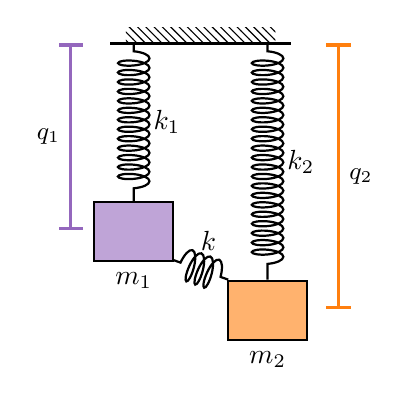
\begin{tikzpicture}[
    black,
    thick,
    spring/.style={decoration={
        coil,
        aspect=0.3, 
        segment length=1.2mm, 
        amplitude=2mm, 
        pre length=1mm,
        post length=1mm}}]
 
% Supporting structure
\fill [pattern = north west lines] (-1.8, 0) rectangle (0.1, .2);
\draw[thick] (-2,0) -- (.3,0);
 
% Mass 1
    \node[draw,
    fill=mpurple!60,
    minimum width=1cm,
    minimum height=0.75cm,
    anchor=north,
    label=south:$m_1$] (mass1) at (-1.7,-2) {};

    % Mass 2
\node[draw,
    fill=morange!60,
    minimum width=1cm,
    minimum height=0.75cm,
    anchor=north,
    label=south:$m_2$] (mass2) at (0,-3) {};
 
% q1 arrow
\draw[very thick,
    mpurple,
    |-|] (-2.5, 0) -- (-2.5,-2.375)
    node[midway,left]{\small \color{black} $q_1$};
 
% q2 arrow
\draw [very thick,
    morange,
    |-|] (0.9, 0) -- (0.9, -3.375)
    node[midway, right]{\small \color{black}$q_2$};
 
% Spring 
\draw
[spring, decorate] (-1.7,0) -- (-1.7,-2) 
    node[midway,right=0.12cm,black]{$k_1$}; 

    % Spring 
\draw
[spring, decorate] (0,0) -- (0,-3) 
    node[midway,right=0.12cm,black]{$k_2$}; 

    \draw
    [spring, decorate] (-1.2,-2.75) -- (-.5,-3) 
        node[midway, above=0.12cm, xshift=.1cm, black]{$k$}; 

\end{tikzpicture}
 
\end{document}